% vim:ts=4:sw=4
% Copyright (c) 2014 Casper Ti. Vector
% Public domain.

\chapter{引言}
% 中文测试文字。
\section{研究背景}
\subsection{高速公路交通研究背景}

高速公路网络已经成为支撑国家经济发展、服务群众生活、保障国家安全的战略资源和设施。截止2016年底,我国公路通车总里程达到457万公里,其中高速公路12万公里,2017年将新增4500公里,是世界上规模最大的高速公路网络(如图\ref{gaosugonglu}所示)。 

				\begin{figure}[h]
				\centering
						\begin{minipage}{0.8\linewidth}
							\centering
							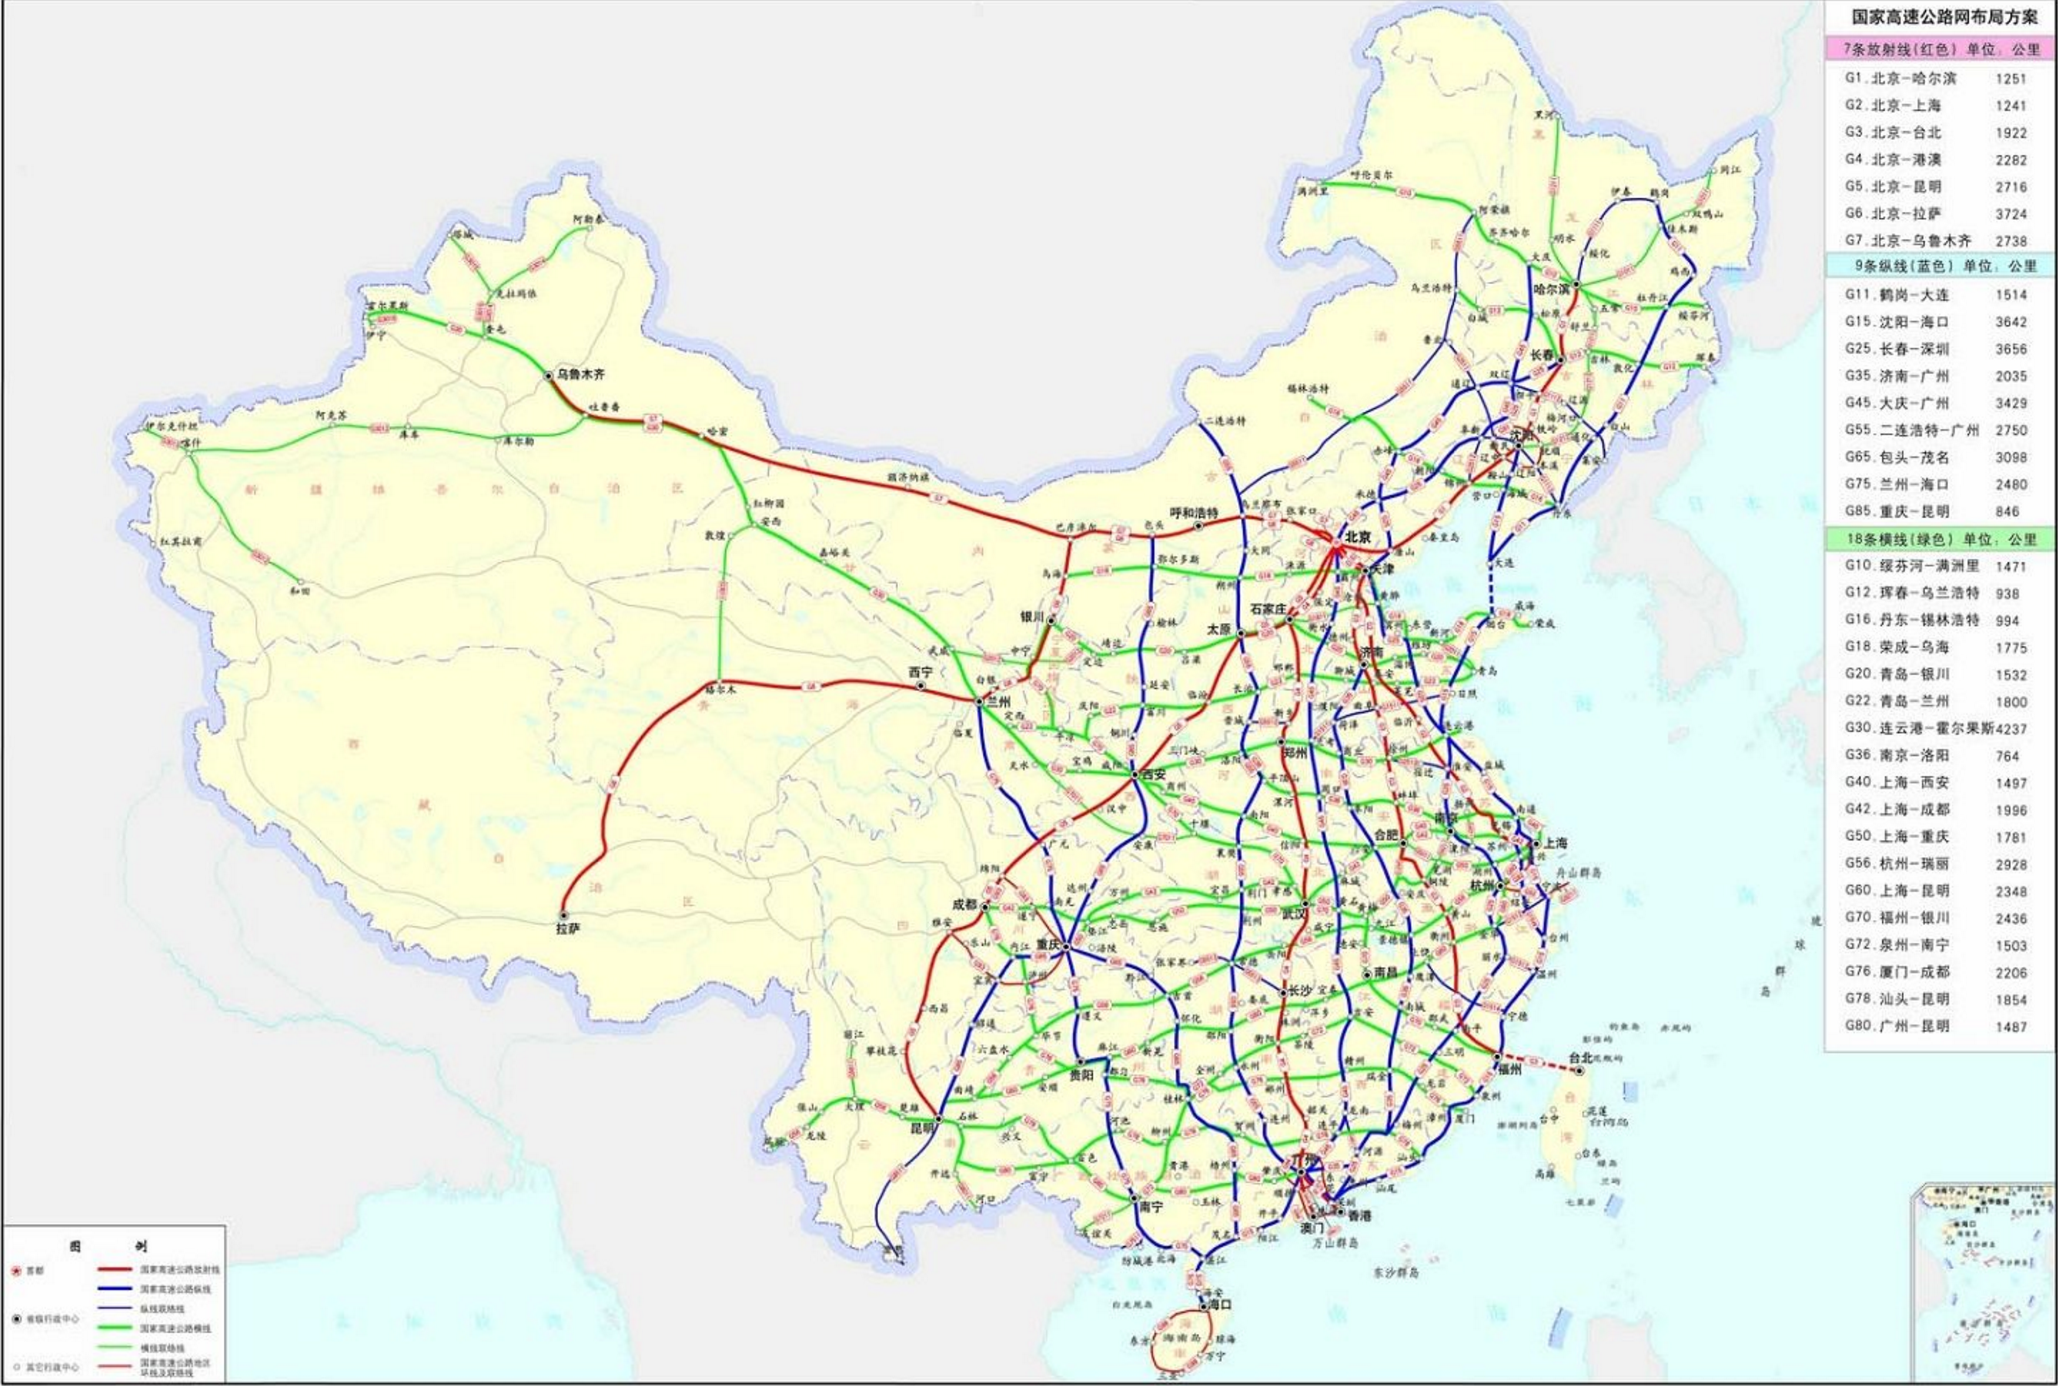
\includegraphics[width=4.4in]{picture/gaosugonglu}
							\caption{fig1}
							\label{gaosugonglu}
						\end{minipage}%\
				\end{figure}

随着中国经济的快速发展,人们生活水平的不断提高,居民的出行和货物运输的数量也在逐渐增加。交通系统是人类活动不可缺少的一部分。据估计,每天平均有40\%的人口在路上花费至少1小时。近几年来,人们变得越来越依赖于交通系统,对于交通系统管理人员来说,机遇和挑战共存。首先,交通拥堵已成为一个日益严重的问题。全球范围内的道路上的车辆增加,根据调查,截止至2016年初,北京共有544万辆车,比2014年初增加了50万辆。这些激增的车辆会对道路系统产生严重的压力,极大的增加拥堵以及拥堵后的损耗。拥堵会导致燃油消耗增加,空气污染,以及实施公共交通计划的困难。车流流量过多时,交通事故风险与交通运输系统中的膨胀增加,交通事故之后的恢复时间与恢复代价也会急剧增加。在中国,2009年的交通事故死亡人数约有7万人,在2015年达到9万人。美国联邦公路管理局公布的报告显示,发生在城市的交通事故约占所有拥堵延误的50\% - 60\%。毫无疑问,如何高效处理交通事故和预测事故发生点,一旦世故发生,最大限度地减少其影响是一个核心问题。由于资源相对有限,尤其是中国高速公路正在逐渐走向免费,因此很难有预算全面建立新的基础设施。同时,运输系统的有效性也越来越依赖于一个国家的处理紧急情况的能力(例如,大规模疏散和安全增强)。一个国家的技术竞争力,其经济实力和生产能力,在很大程度上取决于其交通系统性能。随着高速公路的不断发展,各类维护高速公路的需求也都被一一提出,示例如下:

1)人员分配。最典型的是今年五一,山东高速管理人员联合曲阜路政大队、济宁京台高速交警大队、项目部制定有针对性的应急预案,根据历史的交通信息,负责做好恶劣天气、旅游高峰车流量饱和、突发事件引起交通阻塞的应急处理。安排值班人员,落实机械设备和应急物资准备,一旦发生突发事件,迅速启动,切实做好节日期的保畅工作。

2)安全管理。面对节日期间可能出现的状况,高速公路养护所需要在节日前期组织开展道路安全隐患检查活动:一是对管段路段进行安全隐患排查,发现问题立即落实整改;二是加强春季防火工作的管理,及时清理桥涵构造物下的易燃物品,对边坡、中央分隔带进行打草、苗木修剪,对匝道圈进行专人看护,安排养护员负责所辖路段的防火报警工作。

3)基础设施建设。交通的基础设施建设主要包括交通轨道交通设施建设、停车场设施建设等。交通基础设施包括为交通系统保障安全正常运营而建设的公路、轨道、隧道、高架道路、车站、通风亭、机电设备、供电系统、通信信号、道路标线等设施。

4)高新设施建设。目前越来越多的新技术涌现,比如说最近成都绕城高速公路的部分路段的养护施工采用了新技术——“就地热再生”。这是目前国际上先进的沥青路面施工技术,具有高效、优质、环保、节约的特点,施工过程中采用的是单车道施工方式,施工时占用的工作面小,不中断交通,施工完半小时路面温度降至50摄氏度即快速开放交通。同时就地热再生施工相比传统工艺,在温室气体排放量方面,每施工1万平方米可减少二氧化碳排放26吨,在资源的利用率方面,每施工1万平方米利用废旧沥青混合料960吨,节约新沥青料600吨。就地热再生方法在节能环保、废旧沥青再利用方面的优势在本次绕城高速施工中显现。

上述需求中有一个共性的问题,那就是如何找出高速公路网络中最重要的路段,然后针对这些重要路段,进行针对性管理。高速公路的变化日新月异,根据经验很难非常准确的预估出所有关键路段。亟需提出一套适用于大规模路网的高速公路的关键路段挖掘识别系统。在识别高速公路网络中关键路段的前提下,我们可以进行有效的人员分配,避免人员浪费;可以针对高危路段进行安全管理,减少事故风险;可以针对具有强烈需求的路段进行基础设施建设,避免资源浪费,也可以研究当关键路段因为施工等原因停滞时,如何将影响减少到最小。

本文提出的面向高速公路的关键路段挖掘模型就是一种为了满足上述需求而提出的模型。本文将重点分析高速公路网络的网络特点,以路段/网络运行效率模型为评价标准,在宏观层面上提出一种高速公路重要节点的挖掘模型,同时分析其模型性质,提出一种优化策略。从整体路网的流量角度提出适用于中国高速公路的大规模高速公路网络的关键路段识别算法。

本文针对高速公路进行关键节点挖掘,主要基于高速公路收费数据,并得到如下项目的支持:

1)



\subsubsection{网络性}
    纵横交错的道路构成了复杂的交通路网,这使得交通系统具有了网络性质。网络中,不同的收费站构成了节点,相邻收费站之间的道路构成了网络中的边,节点之间通过车辆来交流。高速公路网络化,使得交通系统中的车流行为更加复杂,这对交通研究方法提出了更高的要求。网络化所引发的复杂性在于,路网中不同空间位置的交通流行为并非孤立产生,而是相互间存在着紧密关系,路网愈加庞大,关系愈为复杂。两个路网中不同空间位置的交通流之间存在着紧密关联,例如较多的车流从某些特定的入口进入路网,又从某些特定的出口流出路网,并且不同出口共享着某些车流来源。然而,传统的以单位置点为研究对象的交通流分析方法并不能有效利用车流之间的关联信息,因此它们已经无法再适用于网络化的交通系统。交通流之间的关联性促生了从路网视角进行全局交通流分析的需求,要求将路网中多节点的交通流行为同时进行学习。

\subsubsection{小世界特性}

    小世界特性(Small world theory)又被称之为是六度空间理论或者是六度分割理论(Six degrees of separation)。小世界特性指出:社交网络中的任何一个成员和任何一个陌生人之间所间隔的人不会超过六个。在高速公路网络中,小世界特性的表现有所不同:网络中绝大部分车辆的跳数(车辆旅行途中经过的道路数量)小于6个.
    
\subsubsection{无标度特性}
				现实世界的网络大部分都不是随机网络,少数的节点往往拥有大量的连接,而大部分节点却很少,节点的度数分布符合幂率分布,而这就被称为是网络的无标度特性(Scale-free)。将度分布符合幂律分布的复杂网络称为无标度网络。在高速公路网络中,统计发现少量节点占有着大多数车辆。(上图)
\subsubsection{社区结构特性}
				人以类聚,物以群分。复杂网络中的节点往往也呈现出集群特性。例如,社会网络中总是存在熟人圈或朋友圈,其中每个成员都认识其他成员。集群程度的意义是网络集团化的程度;这是一种网络的内聚倾向。连通集团概念反映的是一个大网络中各集聚的小网络分布和相互联系的状况。在高速公路网络中,这个特性体现在:高速公路的节点组成一个个社团,这些社团绝大部分车辆都驶向社团内部。
\subsubsection{动态性以及周期性}
				交通路网是一种动态系统,随着时间的变化,其内部的交通流规律与运行模式都在不断变化。交通现象具有周期性,典型的例子是以日为周期的交通流交替运行模式。


\section{研究内容}
    综上所述,本文从交通实际问题的角度出发,针对现有复杂网络关键节点挖掘技术的不足,深入开展下述两项研究内容:
    
		(1)提出一种度量高速公路节点重要性的研究模型,可以在宏观层面反映这些节点对高速公路网络的影响高,挖掘高速公路关键节点
		
		(2)提出一种结合高速公路网络特性的社群划分算法,达到较强的收敛性与低误差。
		
\section{论文结构}
    第一章为绪论,介绍了本文的研究背景,提出了本文的研究内容。第二章
介绍了复杂网络关键节点研究的相关工作,结合交通问题的特点分析了现有方法的优势与不
足。第三章对复杂网络社群划分方法及其相关研究进行了介绍,通过对现有社群划分方法的分类对比,分析了它们的优势与不足。从第四章开始的后续章节将论述本
文的主要研究内容。第四章提出了一种复杂网络关键节点挖掘模型,给出
了详尽的理论分析,并在多个数据集下进行了验证。第五章
提出了一种基于高速公路交通网络的社群划分模型,给出了高效的优化算法和详
尽的理论分析,并在多个数据集下的进行了验证。第六章给出了混合模型在真实交通场景下的应用
实例。第七章给出了全文的总结与未来工作展望。